\subsection{Waveforms Buck Converter, continuous inductor current}\label{2.6}
In deze sectie analyseren we het gedrag van een buck converter die werkt in continue inductorstroommodus. Met behulp van de opgegeven componentwaarden (zie \autoref{tab:component_values16}) simuleren we het convertercircuit om de relatie te observeren tussen de inductorstroom \( I_L \) en andere belangrijke parameters, zoals de uitgangsspanning \( V_{out} \), de spanningspoot \( V_{leg} \), en verschillende stroompaden binnen de converter.

\begin{table}[h!]
\centering
\begin{tabular}{|l|c|}
\hline
\textbf{Component} & \textbf{Value} \\ \hline
Vin & 48 V \\ \hline
L & 100 µH \\ \hline
C & 10 µF \\ \hline
Rout & 10 \(\Omega\) \\ \hline
Fs & 50 kHz \\ \hline
d & 40\% \\ \hline
\end{tabular}
\caption{Component values for the circuit}
\label{tab:component_values16}
\end{table}
\begin{figure}[h!]
    \centering
    \begin{subfigure}[b]{0.5\linewidth}
        \centering
        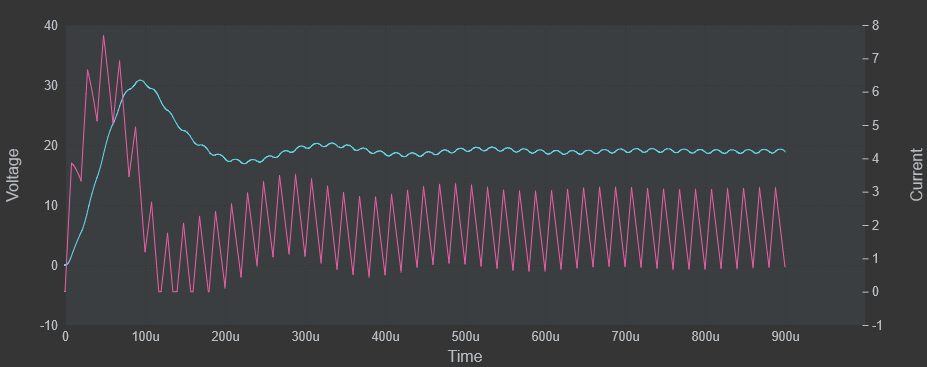
\includegraphics[width=\linewidth]{img/hfd2/IL-Vout.png}
        \caption{\(I_{L}\) and \(V_{out}\)}
        \label{fig:Waveform_IL_Vout}
    \end{subfigure}
    \hfill
    \begin{subfigure}[b]{0.5\linewidth}
        \centering
        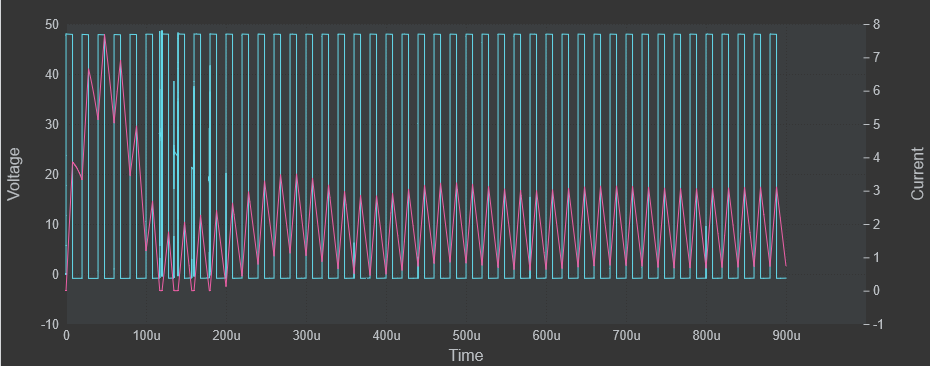
\includegraphics[width=\linewidth]{img/hfd2/IL-Vleg.png}
        \caption{\(I_{L}\) and \(V_{leg}\)}
        \label{fig:Waveform_IL_VLeg}
    \end{subfigure}
    \caption{Waveforms}
    \label{fig:Waveforms}
\end{figure}

Met deze waarden ingevoerd in de simulatie genereren we een reeks golfvormen die de inductorstroom \( I_L \) in relatie tot andere circuitcomponenten illustreren. Figuur \ref{fig:Waveforms} toont de golfvormen van \( I_L \) naast de uitgangsspanning \( V_{out} \) en de spanningspoot \( V_{leg} \). Daarnaast geeft Figuur \ref{fig:Waveforms_IL_all} gedetailleerde vergelijkingen van de golfvormen van \( I_L \) met de drain-source stroom \( I_{DS} \), diodestroom \( I_{D} \), condensatorstroom \( I_{C} \), weerstandsstroom \( I_{R} \), en ingangsstroom \( I_{\text{in}} \). Deze vergelijkingen helpen om de stroomrichting en spanningsniveaus door het circuit heen te visualiseren.

\begin{figure}[h!]
    \centering
    \begin{subfigure}[b]{0.45\linewidth}
        \centering
        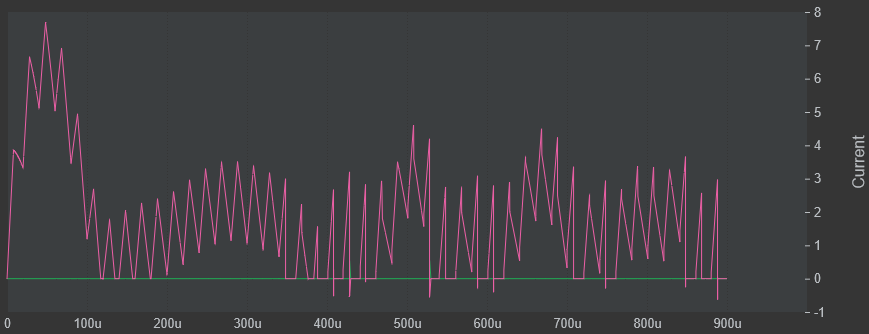
\includegraphics[width=\linewidth]{img/hfd2/IL-IDS.png}
        \caption{Waveform of \(I_{L}\) and \(I_{DS}\)}
        \label{fig:Waveform_IL_IDS}
    \end{subfigure}
    \hfill
    \begin{subfigure}[b]{0.45\linewidth}
        \centering
        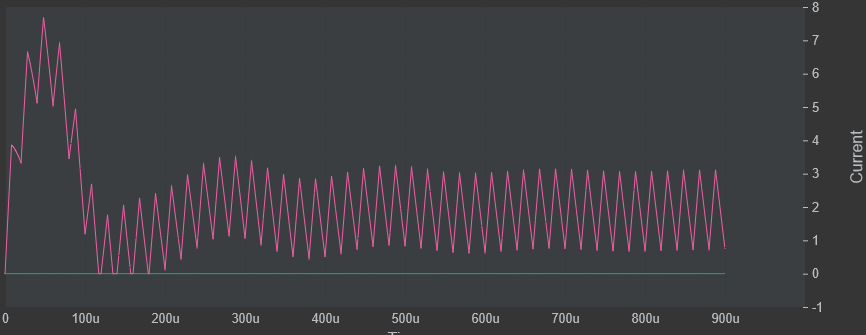
\includegraphics[width=\linewidth]{img/hfd2/IL-ID.png}
        \caption{Waveform of \(I_{L}\) and \(I_{D}\)}
        \label{fig:Waveform_IL_ID}
    \end{subfigure}
    
    \begin{subfigure}[b]{0.45\linewidth}
        \centering
        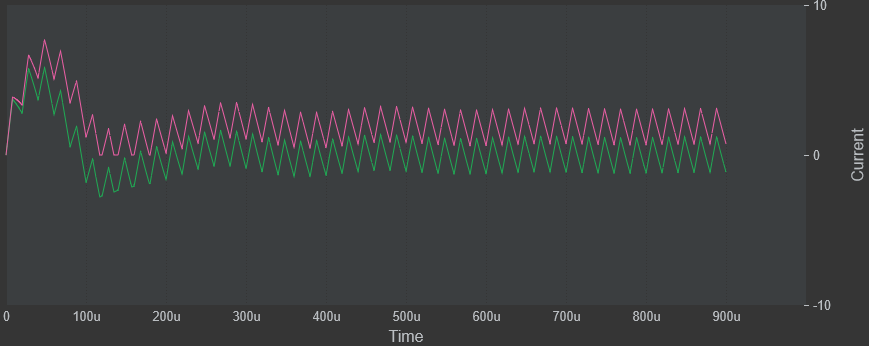
\includegraphics[width=\linewidth]{img/hfd2/IL-IC.png}
        \caption{Waveform of \(I_{L}\) and \(I_{C}\)}
        \label{fig:Waveform_IL_IC}
    \end{subfigure}
    \hfill
    \begin{subfigure}[b]{0.45\linewidth}
        \centering
        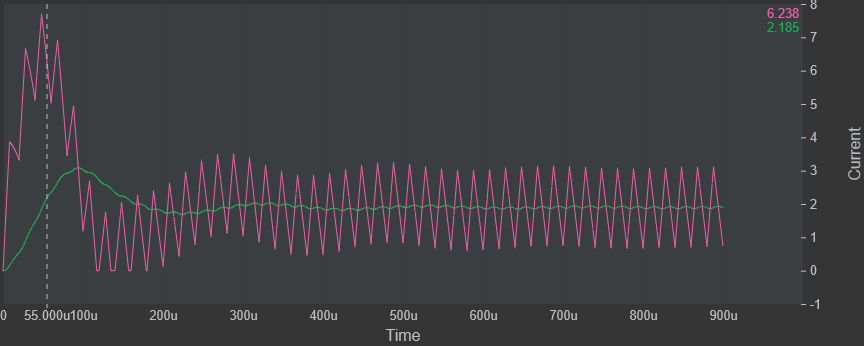
\includegraphics[width=\linewidth]{img/hfd2/IL-IR.png}
        \caption{Waveform of \(I_{L}\) and \(I_{R}\)}
        \label{fig:Waveform_IL_IR}
    \end{subfigure}
    
    \begin{subfigure}[b]{0.45\linewidth}
        \centering
        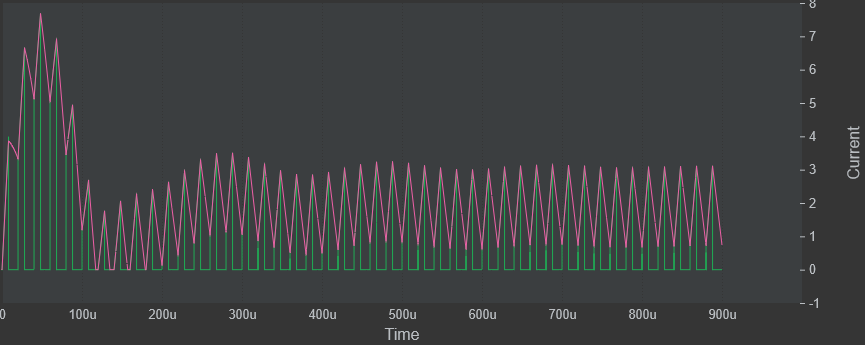
\includegraphics[width=\linewidth]{img/hfd2/IL-Lin.png}
        \caption{Waveform of \(I_{L}\) and \(I_{\text{in}}\)}
        \label{fig:Waveform_IL_Lin}
    \end{subfigure}
    
    \caption{Waveforms comparing \(I_{L}\) with various parameters: \(I_{DS}\), \(I_{D}\), \(I_{C}\), \(I_{R}\), and \(I_{\text{in}}\)}
    \label{fig:Waveforms_IL_all}
\end{figure}

Elke golfvorm biedt inzicht in het schakelgedrag, de energieoverdracht en de verliezen binnen de buck converter onder omstandigheden van continue inductorstroom, wat cruciaal is voor het begrijpen van de efficiëntie en stabiliteit van de converter.